\section{Visual Search Techniques}
\label{sec:visual_search_techniques}

\subsection{Evaluation Methods}
\label{sec:eval_methods}

It is crucial to assess an image retrieval system in order to fully understand its performance. A variety of metrics
and approaches are used to assess an image retrieval system's performance. The experimental findings in this paper
are evaluated using precision and recall metrics.

Precision of a system is determined by counting the number of retrieved items that are actually relevant.
It is the proportion of all images retrieved that are relevant to all images retrieved. A high precision value means
that a large proportion of the retrieved items are indeed relevant.

\begin{equation}
  Precision = \frac{\text{Number of Relevant Items Retrieved}}{\text{Total Number of Items Retrieved}}
\end{equation}

Recall measures how well the system can identify and retrieve all relevant images. It is the ratio of relevant images
retrieved to the total number of relevant images in the database. A higher recall indicates that the system can find
a larger proportion of relevant images.

\begin{equation}
  Recall = \frac{\text{Number of Relevant Items Retrieved}}{\text{Total Number of Relevant Items}}
\end{equation}

\subsection{Feature Extraction}
\label{sec:feature_extraction_details}

Images are 2-D arrays containing the pixel intensities for each color channel. However it is difficult to compare images
based on their pixel intensities. This is because the pixel intensities are not aware of the subject in the image and
fail to explain the subject's scale, shape, etc. Feature extractors are functions that can effectively analyse most of
the image's features and then, output descriptors which are used to compare images.

\subsubsection{Average Color}
\label{sec:average_color}

Average color is a very simple descriptor that outputs an array of three numbers representing the mean intensities of
the red, green and blue channels of the image. However, this descriptor does not represent the subject of the image or
its shape and edge information. The average color descriptor ignores a lot of information and as a result it is only
used as a sub-descriptor (see section~\ref{sec:spacial_grid} for applications of the Average Color descriptor).

\subsubsection{Global Color Histogram}
\label{sec:global_color_histogram}

The Average Color descriptor outputs the exact mean of the image's intensity values. This does not work well in
real-world problems because the intensity values in an image can always vary depending on the lighting conditions of
the scene. The Global Color Histogram is a descriptor that outputs a histogram of color distributions. The descriptor
defines similarity as "similar overall color". This makes the descriptor tolerant to slight intensity variations
between images.

The Global Color Histogram \cite{colorhistforcbir} descriptor outputs a descriptor that represents the overall
color distribution of the image. The color histogram for a image is calculated by quantizing the color space into
several bins. Equation \ref{eq:rgb_quantization} shows how the RGB intensities of the image are quantized, where $q$
is the Quantization level. The pixels of the image are then categorized into these bins, which are then counted to
output the color histogram descriptor.

\begin{equation}
  r' = floor(r \times \frac{q}{256}) \qquad g' = floor(g \times \frac{q}{256}) \qquad b' = floor(b \times \frac{q}{256})
  \label{eq:rgb_quantization}
\end{equation}

\subsubsection{Edge Histogram}
\label{sec:edge_histogram}

Edge Histogram descriptor considers two images similar if they have similar edge orientations. The descriptor uses an
edge detection algorithm to find significant changes in intensity (usually edges). The edges are then thresholded to
include only the prominent edges in the image. A histogram is calculated based on the orientation of these edges.
Edge Histogram can represent texture information in an image and is often used in combination with other descriptors.
This paper uses Sobel \cite{digitalimageprocessing} for edge detection. Figure \ref{fig:sobel} shows how the Sobel
filter extracts edge information.

\begin{figure}[htbp]
  \begin{center}
    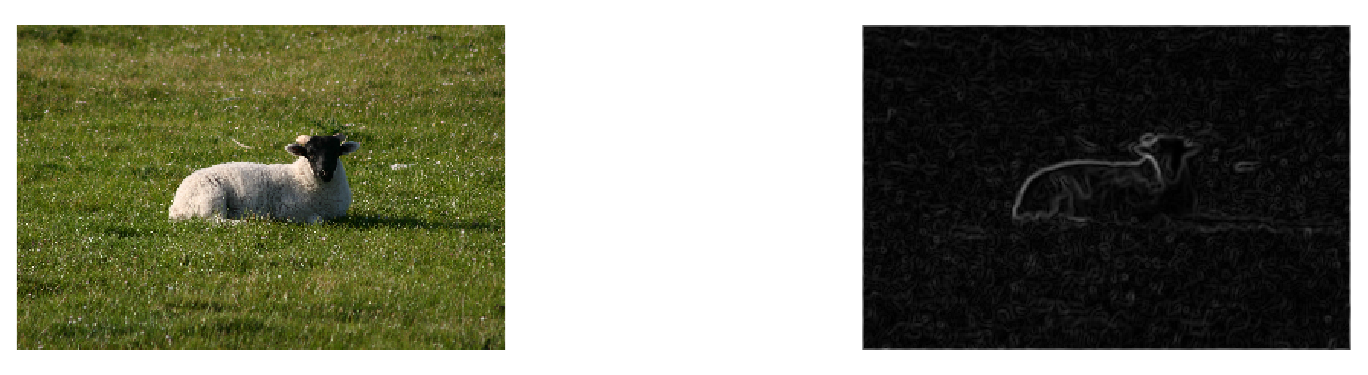
\includegraphics[width=0.75\textwidth]{./assets/plots/sobel.png}
    \caption{Image followed by a visualization of its edge magnitudes}
    \label{fig:sobel}
  \end{center}
\end{figure}


\subsubsection{Spacial Grid}
\label{sec:spacial_grid}

All the descriptors mentioned above do not take the spacial information from the image into consideration. This means
the intensity values on the top left of the image cannot be differed from similar intensities values on the bottom
right of the image. Spacial Grid solves this problem by splitting the image into a 2-D grid and calculating descriptors
for each cell.

Spacial grid can be used with many other descriptors to make the resulting descriptor sensitive to spacial information.
A suitable descriptor is used on every cell in the image grid and the resulting grid of descriptors is flattened into
a 1-D array. This paper explores the use of spacial grid with Average Color, Edge Histogram and a combination of both.

\subsubsection{Convolutional Neural Network}
\label{sec:conv_nn}

Convolutional Neural Networks or CNNs are powerful architectures that can process images highly effectively for
computer vision tasks such as image classification, object detection and feature extraction. CNNs automatically extract
image features in the first few layers of its network. The outputs of these layers can be used as an image descriptor.
For example, in this paper a CNN known as AlexNet \cite{krizhevsky2012imagenet} was used as a feature extractor (using
outputs of AlexNet's "fc7" layer).

\subsection{Similarity Measure}
\label{sec:similarity_measure_details}

The descriptors from feature extractors can be compared to measure the similarity between two images. Image retrieval
systems then sort images based on this measure. There are various similarity measures, however this paper only uses
L1, Euclidean and Mahalanobis distance functions as similarity measures.

\subsubsection{L1 Distance (Manhattan Distance)}
\label{sec:l1_dist}

The L1 distance, also known as the Manhattan distance or City Block distance, is a measure of the absolute differences
between the coordinates of two points in a multidimensional space. The L1 distance between two points $a$ and $b$
is calculated with

\begin{equation}
  L1~Distance(a,b) = \sum_{i=1}^{n} | a_i - b_i |
  \label{eq:l1_distance}
\end{equation}

\subsubsection{Euclidean Distance (L2 Norm)}
\label{sec:euclidean_dist}

Euclidean distance is a measure of the straight-line distance between two points in Euclidean space. It is the most
common metric used to quantify the dissimilarity or similarity between two vectors. The Euclidean distance between
two points is calculated with

\begin{equation}
  Euclidean~Distance(a,b) = \sqrt{\sum_{i=1}^{n}  (a_i - b_i)^2}
  \label{eq:euclidean_distance}
\end{equation}

\subsubsection{Mahalanobis Distance}
\label{sec:mahalanobis_dist}

Mahalanobis distance is a metric used to measure the distance between a point and a distribution, taking into
account the correlations between variables. It is a generalized form of distance that considers the covariance
structure of the data. Mahalanobis distance is particularly useful when dealing with multivariate data, where the
variables are correlated. It is used often with PCA, a dimensionality reduction technique because it respects the
structure of the data.

The Mahalanobis distance, $D_M$ is calculated with

\begin{equation}
  D_M(a, b) = \sqrt{ \sum_{i=1}^{n} \frac{(a_i - b_i)^2}{v_i} }
  \label{eq:mahalanobis_distance}
\end{equation}

where, $v_i$ is the eigen value of the $i^{th}$ space.

\subsection{Principal Component Analysis}
\label{sec:pca}

A popular dimensionality reduction technique in statistics and machine learning is principal component analysis, or
PCA. It transforms a dataset into a lower dimensional coordinate system, emphasizing directions of maximum variance.
The process for dimensionality reduction using PCA involves centering the data, calculating the covariance matrix,
selecting the principal components, determining the eigenvectors and eigenvalues, and producing a projection matrix.
PCA keeps important information while reducing dimensionality by projecting the data into this subspace. PCA is used
for image compression, signal processing, and machine learning for feature reduction and analysis.
